\documentclass{beamer}
\usetheme{Warsaw}
%\usetheme[progressbar = frametitle]{metropolis}
%\setbeamertemplate{frame numbering}[fraction]
% latexcolor.com for g=rgb values
\definecolor{wisteria}{rgb}{0.79, 0.63, 0.86}
\usecolortheme[named = wisteria]{structure}
\title[Linux]{A friendly introduction to Open Source Linux}
\subtitle{}
\author{Nikita Masand}
\institute{\large\textbf{VJTI}}
\date{}
\begin{document}
\begin{frame}
\titlepage
\end{frame}
\begin{frame}{Contents}
\begin{table}[]
    \centering
     \caption{Table of Contents}
    \begin{tabular}{l|c|}
        Sr. no & Content \\
        \hline \hline
       1 & Asking the difference between Linux and Ubuntu \\
       2 & Why Linux? \\
       3 & What is Linux? \\
       4 & Linux Architecture\\
       5 & Kernel\\
       6 & Components of Architecture\\
       7 & Features\\
       8 & Thank you
       
    \end{tabular}
   
    \label{tab:my_label}
\end{table}
    
\end{frame}

\begin{frame}{Can someone answer this?}\vspace{10pt}
The difference between Linux and Ubuntu is 
\only<1>{\line(1,0){50}}
\only<2>{\textcolor{green}{
Linux is the name of the core component of the operating system. It is called a kernel. Ubuntu is one distribution that uses the Linux kernel.
}}

Ubuntu uses 
\only<1>{\line(1,0){50}}
\only<2>{\textcolor{magenta}{linux}}
\,kernel while windows use 
\only<1>{\line(1,0){50}}
\only<2>{\textcolor{magenta}{hybrid NT kernel}}
\,kernel \\[10pt]

\begin{block} {Therefore there is a need to know what linux kernel is}
\vspace{0.5 em}
The kernel manages input, output, memory, and processing.The collection of utilities and interfaces is called a distribution.

\end{block}
\end{frame}

{
\usebackgroundtemplate{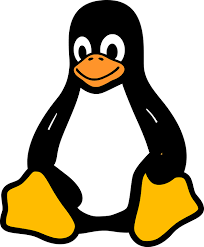
\includegraphics[width=\paperwidth]{linux.png}}
\begin{frame}[t]{Why Linux?}\vspace{10pt}
\textcolor{green}{If you’re a refugee from Windows, you may be finding the Linux world slightly confusing. Never fear! Linux is not some scary, difficult to use monster,it’s actually becoming user friendly every day.}
\newline
\newline
\begin{block}{Linux is everywhere}
\vspace{0.5 em}
Linux is used from smartphones to cars, supercomputers and home appliances.It runs most of the Internet, the supercomputers making scientific breakthroughs, and the world\'s stock exchanges. But before Linux became the platform to run desktops, servers, and embedded systems across the globe, it was (and still is) one of the most reliable, secure, and worry-free OS available.
\end{block}
\end{frame}
}


\begin{frame}{But What is Linux?}\vspace{10pt}
   \begin{enumerate}
   \item An operating system is an interface between the user of a computer and the computer hardware.
   
    \item Linux is a family of free and open-source software OS based on the Linux kernel,an OS kernel first released on September 17, 1991 by Linus Torvalds.
    
    \item It is written majorly in the C language
\end{enumerate} 
\end{frame}
\begin{frame}[t]{Linux Architecture}
    \begin{SCfigure}
    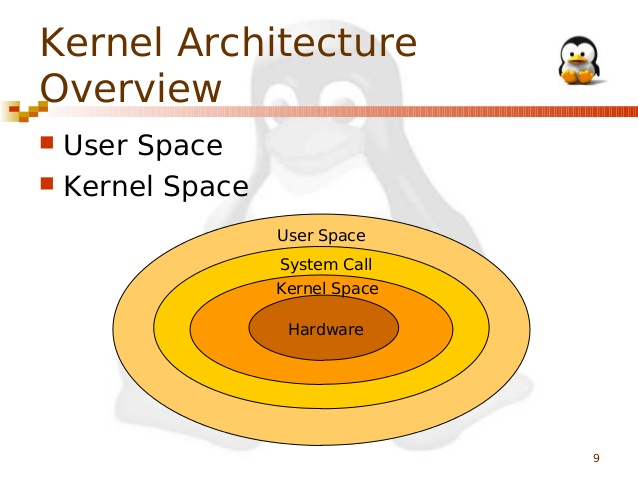
\includegraphics[width = \paperwidth]{linux-kernel-architecture-9-638.jpg}
    \caption{Components}
    \end{SCfigure}
\end{frame}

\begin{frame}{Explaining Kernel}
\begin{enumerate}[A]
    \item  The kernel is the core part of the operating system, which is  responsible for all the major activities of the LINUX operating system.
    \item The kernel offers the required abstraction to hide  application programs or low-level hardware details to the system. 
    \item The types of Kernel are:
    \begin{enumerate}
        \item Monolithic Kernel
        \item Micro kernels
        \item Exo kernels
        \item Hybrid kernels
    \end{enumerate}
\end{enumerate}
    
\end{frame}
}
\begin{frame}{Describing Components}
    \begin{table}
    \caption{Other Linux components}
\begin{tabular}{l | c | }
Component & Description \\
\hline \hline
System library  & used to implement the functionality of the OS   \\ 
Utilityprogram &do individual, and specialized-level tasks \\
Hardwarelayer & peripheral devices such as RAM, HDD, CPU \\
Shell & take command from user and executes kernel functions. 
\end{tabular}

\end{table}
\end{frame}
\begin{frame}{Features of Linux}
    \begin{enumerate}
        \item Portable (Multiplatform)
        \item Open Source
        \item Multiuser
        \item MultiProgramming
        \item Hierarchical File System
        \item Shell
        \item Security
    \end{enumerate}
\end{frame}


\begin{frame}[allowframebreaks] %allow to expand references to multiple frames (slides)

\frametitle{References}
\begin{thebibliography}{}
\bibitem{}https://www.linux.org
\bibitem{}https://www.howtogeek.com/howto/31632/what-is-the-linux-kernel-and-what-does-it-do/
\bibitem{}https://en.wikipedia.org/wiki/Linuxkernel
\bibitem{}https://www.quora.com/WhatisaLinuxKernel
\bibitem{}https://www.computerhope.com/jargon/l/linux-kernel.htm
\bibitem{}https://www.ibm.com/developerworks/library/l-linux-kernel/index.html

\end{thebibliography}
\end{frame}

\begin{frame}{Thank you}
\begin{figure}
    \centering
    
\includegraphics{thankyou.jpg}
    \caption{Thank you}
    \label{fig:my_label}
\end{figure}

\end{frame}
\end{document}